\documentclass[tikz,border=2pt]{standalone}
\usepackage{amsmath}
\usepackage{pgfplots}
\pgfplotsset{compat=1.18}
\usetikzlibrary{arrows.meta,decorations.pathreplacing}
\begin{document}
% Final tableau of Example 6.2 (max 3x1+5x2, x1<=4, 2x2<=12, 3x1+2x2<=18): objective row (0,0 | 0,3/2,1 | 36).
% Slack columns give y = c_B^T B^{-1} = (0,3/2,1); structural columns give the dual surpluses A^T y - c = (0,0);
% the right-hand side is Z = W = 36; the constraint rows give the primal basic solution x3=2, x2=6, x1=2.
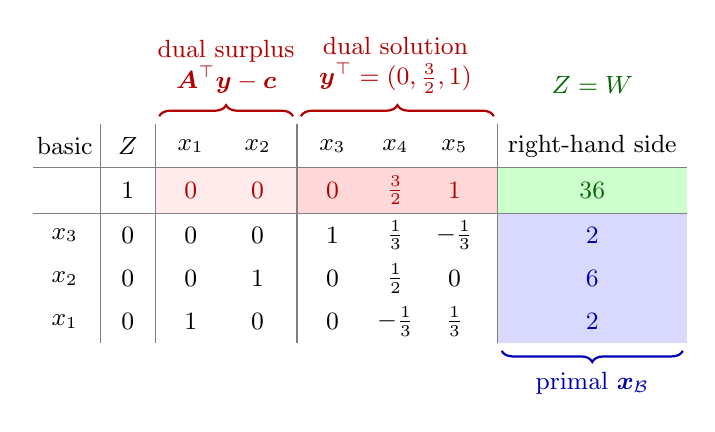
\begin{tikzpicture}[font=\small, >={Latex[length=2mm]}]
  % highlights
  \fill[red!8] (1.15,-0.27) rectangle (2.95,-0.85);
  \fill[red!15] (2.95,-0.27) rectangle (5.5,-0.85);
  \fill[green!20] (5.5,-0.27) rectangle (7.9,-0.85);
  \fill[blue!15] (5.5,-0.85) rectangle (7.9,-2.5);
  % grid
  \draw[gray] (-0.4,-0.27) -- (7.9,-0.27) (-0.4,-0.85) -- (7.9,-0.85);
  \foreach \x in {0.45,1.15,2.95,5.5} \draw[gray] (\x,0.28) -- (\x,-2.5);
  % header
  \node at (0,0) {basic};
  \node at (0.8,0) {$Z$};
  \foreach \j/\x in {1/1.6,2/2.45,3/3.4,4/4.2,5/4.95} \node at (\x,0) {$x_{\j}$};
  \node at (6.7,0) {right-hand side};
  % objective row
  \node at (0.8,-0.56) {$1$};
  \node[red!70!black] at (1.6,-0.56) {$0$};
  \node[red!70!black] at (2.45,-0.56) {$0$};
  \node[red!70!black] at (3.4,-0.56) {$0$};
  \node[red!70!black] at (4.2,-0.56) {$\tfrac{3}{2}$};
  \node[red!70!black] at (4.95,-0.56) {$1$};
  \node[green!40!black] at (6.7,-0.56) {$36$};
  % constraint rows
  \foreach \b/\y/\p/\q/\r/\s/\t/\h in {3/-1.13/0/0/1/{\tfrac{1}{3}}/{-\tfrac{1}{3}}/2, 2/-1.68/0/1/0/{\tfrac{1}{2}}/0/6, 1/-2.23/1/0/0/{-\tfrac{1}{3}}/{\tfrac{1}{3}}/2} {
    \node at (0,\y) {$x_{\b}$};
    \node at (0.8,\y) {$0$};
    \node at (1.6,\y) {$\p$}; \node at (2.45,\y) {$\q$};
    \node at (3.4,\y) {$\r$}; \node at (4.2,\y) {$\s$}; \node at (4.95,\y) {$\t$};
    \node[blue!70!black] at (6.7,\y) {$\h$};
  }
  % readings
  \draw[red!70!black, thick, decorate, decoration={brace, amplitude=4pt}] (1.2,0.38) -- (2.9,0.38);
  \node[red!70!black, anchor=south, align=center] at (2.05,0.55) {dual surplus\\ $\boldsymbol{A}^{\top}\boldsymbol{y}-\boldsymbol{c}$};
  \draw[red!70!black, thick, decorate, decoration={brace, amplitude=4pt}] (3.0,0.38) -- (5.45,0.38);
  \node[red!70!black, anchor=south, align=center] at (4.2,0.55) {dual solution\\ $\boldsymbol{y}^{\top}=(0,\tfrac{3}{2},1)$};
  \node[green!40!black, anchor=south, align=center] at (6.7,0.55) {$Z=W$};
  \draw[blue!70!black, thick, decorate, decoration={brace, amplitude=4pt, mirror}] (5.55,-2.6) -- (7.85,-2.6);
  \node[blue!70!black, anchor=north] at (6.7,-2.75) {primal $\boldsymbol{x}_{\mathcal{B}}$};
\end{tikzpicture}
\end{document}
